\documentclass[manuscript,review,anonymous]{acmart}

\usepackage{luatexja}
\usepackage{luatexja-fontspec}
\usepackage{booktabs}
\usepackage{tabularx}
\usepackage{graphicx}
\graphicspath{{figures/pdf/}}

\setmainjfont[
  BoldFont=HaranoAjiMincho-Bold,
  ItalicFont=HaranoAjiMincho-Regular,
  BoldItalicFont=HaranoAjiMincho-Bold
]{HaranoAjiMincho-Regular}
\setsansjfont[
  BoldFont=HaranoAjiGothic-Bold
]{HaranoAjiGothic-Medium}
\setmonojfont{HaranoAjiGothic-Regular}
\settopmatter{printacmref=true,printccs=true,printfolios=true}
\setcopyright{none}
\acmConference[CHI '27]{Proceedings of the 2027 CHI Conference on Human Factors in Computing Systems}{May 2027}{Barcelona, Spain}
\acmYear{2027}
\copyrightyear{2027}

\newcommand{\term}[1]{\textbf{#1}}
\newcommand{\condition}[1]{\textsf{#1}}
\newcommand{\pct}[1]{#1\%}
\newcolumntype{Y}{>{\raggedright\arraybackslash}X}

\title{生成臨床UIの更新における層間整合性の評価}
\author{Anonymous Author(s)}

\begin{document}

\begin{abstract}
診療を支える生成UIでは、SQLの実行や画面の描画に加え、診療場面に応じた対象患者、項目、期間、情報源の指定が適切な表示まで一貫して保たれる必要がある。本研究は、この過程で情報要求、SQL、実行結果、表示の対応が壊れた状態を層間不整合と定義し、検出・特定・修復する評価基盤を示す。EHRSQL-2024とMIMIC-IV Demoを用いて8種類の不整合を決定的に生成し、局所検査、成果物契約、質問から表示までを結ぶグラフ契約、同じ内容を平坦に保持する平坦契約を比較した。134種類の質問テンプレートから763組の更新前後ペアを作り、6,104回検証した。その結果、局所検査と成果物契約は不整合の100.00\%と48.10\%を受理した。グラフ契約と平坦契約は不整合をすべて拒否し、妥当な更新をすべて受理した。両者の差は0であり、検出を支えたのは保存形式ではなく、シナリオ由来の情報要求から表示までの関係を実行可能な契約として保持したことだった。本評価は利用者便益を直接測っていない。その境界を示したうえで、妥当な臨床UXを評価する前提として情報の来歴を検査する設計を論じる。
\end{abstract}

\begin{CCSXML}
<ccs2012>
  <concept>
    <concept_id>10003120.10003121</concept_id>
    <concept_desc>Human-centered computing~Human computer interaction (HCI)</concept_desc>
    <concept_significance>500</concept_significance>
  </concept>
  <concept>
    <concept_id>10003120.10003123.10011760</concept_id>
    <concept_desc>Human-centered computing~Interactive systems and tools</concept_desc>
    <concept_significance>300</concept_significance>
  </concept>
</ccs2012>
\end{CCSXML}

\ccsdesc[500]{Human-centered computing~Human computer interaction (HCI)}
\ccsdesc[300]{Human-centered computing~Interactive systems and tools}

\keywords{生成ユーザーインターフェース, データ駆動型UI, 電子カルテ, 整合性検査, 増分更新, 追跡可能性}

\maketitle

\section{はじめに}

医療者に役立つ画面は、診療場面によって変わる。術前外来では一時点の広い情報を集約する一方、術後フォローでは限られた項目の推移を追う。同じ電子カルテでも、必要な項目、時間範囲、情報源、表示方式は一様ではない。生成UIには、SQLの生成にとどまらず、診療タスクに必要な情報を確認しやすい形で医療者へ返す役割がある。

この目的に対し、従来の技術検査には空白がある。SQLの構文や実行、結果スキーマ、UIコード、画面描画は個別に確認できる。しかし、各成果物が正常でも、SQLだけが別患者を参照する、期間条件だけが外れる、更新前の結果が残る、表示部品が別のデータを参照するといった誤りは起こり得る。SQLの正答率が上がっても、その後の実行、接続、表示まで同じ要求が保たれなければ、医療者へ返る情報は正しくならない。

本稿では、診療場面から定めた情報要求と、最終的に表示される情報の対応が、途中の成果物境界で壊れた状態を\term{層間不整合}と呼ぶ。生成臨床UIの品質を、情報要求から表示までの過程として捉える。ここでいう正しさは医学的判断全体の正しさではない。定められた患者、項目、期間、集約、情報源、表示方式、接続、版が、更新後も一貫していることである。

生成・編集可能なUIの研究では、タスクモデルや意味表現を介して自然言語要求とUIを結ぶ方法が示されている。Jellyは、変化する情報タスクをタスク駆動データモデルとして保持し、自然言語と直接操作による更新を支える\cite{cao2025jelly}。Bridging Gulfsは、設計意図の意味表現を利用者の入力と生成UIの間に置き、解釈を確かめながら生成できるようにする\cite{park2026bridging}。SimStepは複数のタスクレベル表現を使い、生成結果の前提を段階的に確認・修正できるようにする\cite{kaputa2026simstep}。これらは中間表現の価値を示す一方、データ取得を伴うUIの増分更新で、情報要求から表示までのどの関係が壊れ、どの検査で見つかるかを同一候補上で比較していない。

そこで本研究は、生成臨床UIの更新における層間不整合を評価する基盤を構築した。臨床情報要求と正解SQLには、EHRSQL-2024\cite{lee2024ehrsql}を用いる。正解SQLを公開デモ用のMIMIC-IV Clinical Database Demo v2.2\cite{johnson2023mimic}上で実行し、基準となるデータ駆動型UIを作る。そこへ対象患者、対象項目、期間、集約方法、情報源、表示方式、データと表示の接続、更新後に残る古い結果という8種類の不整合を一つずつ入れる。候補生成とは独立した処理で正解を判定し、同じ候補を4種類の検査条件へ入力する。この評価は、妥当な臨床UXを生成する過程のうち、要求どおりの情報が表示へ届くという必要条件を測る。

本研究では次の問いに答える。

\begin{description}
  \item[RQ1] 定義した8種類のうち、SQLや表示部品を一つずつ確認しても通過する情報の誤りはどれか。
  \item[RQ2] 局所検査、成果物ごとの契約、質問から表示までをまとめて確認する契約では、不整合の見逃し、妥当な更新の受理、問題箇所の特定がどう異なるか。
  \item[RQ3] 検査で特定した問題を一回だけ自動修復すると、どの範囲を直せるか。
\end{description}

固定した評価方法でテスト分割を一度だけ実行した結果、134種類の質問テンプレートから763組の更新前後ペアを作った。妥当候補と不整合候補を4条件で検査し、合計6,104回の評価を得た。局所検査は不整合763件をすべて受理し、成果物契約も367件を受理した。質問から表示までを結ぶグラフ契約と、同じ対応内容を一枚の平坦な表に保持する平坦契約は、不整合をすべて拒否し、妥当候補をすべて受理した。両者は判定、問題箇所の特定、一回の修復で同じ結果だった。この一致は、グラフという保存形式に検出上の優位性があるという予想を支持しない。層をまたぐ意味関係を明示し、実行可能な契約として検査したことが結果を分けた。

本稿の貢献は次の五点である。

\begin{itemize}
  \item 診療シナリオごとに情報要求と妥当な表示が変わることを踏まえ、生成臨床UIの評価範囲を、タスク定義の医学的妥当性、層間整合性、利用者による確認に分けた。
  \item データ駆動型UIの増分更新で起こる情報の誤りを、患者、項目、期間、集約、情報源、表示方式、接続、古い結果の8種類として操作可能に定義した。
  \item 公開デモデータ上で不整合を決定的に生成し、候補生成とは独立したオラクルで確認する再現可能な評価方法を示した。
  \item 同じ候補に4種類の検査条件を適用し、個別成果物の妥当性だけでは層間整合性を保証できない範囲を定量化した。
  \item 同じ検査内容を持つグラフ契約と平坦契約が同じ結果を得た。この否定的結果から、生成UIに必要なのは特定の保存形式ではなく、検査可能な層間関係であるという設計上の含意を導いた。
\end{itemize}

本評価は技術評価であり、診療シナリオ自体の医学的妥当性、臨床上の安全性、診療判断の正確さ、使いやすさ、認知負荷、臨床転帰を評価していない。この境界を保ちつつ、情報抽出と表示の整合性が利用者価値へ至る前提であることを論じる。

\section{関連研究}

\subsection{生成・編集可能なUI}

生成UIの研究は、自然言語や例示から画面を生成する段階から、生成物を利用者が理解し、編集し、再利用できる段階へ広がっている。DirectGPTは、会話に加えて生成物そのものを直接操作し、参照解決を支えることで、生成AIとの反復的な作業を扱った\cite{masson2024directgpt}。DynaVisは、可視化の生成と編集を対話的に行い、生成されたUI上の操作を自然言語対話と組み合わせた\cite{vaithilingam2024dynavis}。これらの研究は、生成物を継続的に変更できる対話対象として扱う。

更新可能性を支えるため、中間表現を導入する研究もある。Jellyは、タスク駆動データモデルを生成UIの背後へ置き、タスクの変化をデータと画面へ反映する\cite{cao2025jelly}。Bridging Gulfsは、意味表現を通じて利用者の意図、生成モデルの解釈、出力UIの隔たりを小さくする\cite{park2026bridging}。SimStepは、概念、シナリオ、学習目標、UIのグラフを分け、人が各段階の仮定を編集できるようにする\cite{kaputa2026simstep}。これらの設計では、中間表現が検査や修正の接点になる。

本研究は、より狭い問いを扱う。比較対象は、更新前後でデータの意味関係が保たれたかである。中間表現を利用するが、グラフ形式そのものは貢献として扱わない。同じ関係を平坦な形式でも表し、検出結果を比較することで、形式と確認内容を分けて評価する。

\subsection{人と生成システムの協働における検査と修正}

生成システムの利用者は、出力を単純に採用または拒否するだけではない。Ignore, Trust, or Negotiateは、生成AIの提案を利用者が無視、信頼、交渉しながら取り込む過程を示し、提案の不確実さや根拠を扱える相互作用の必要性を論じた\cite{sivaraman2023ignore}。生成UIでも、エラー表示だけで更新全体を拒否するより、どの関係が壊れ、何を修正すると影響がどこへ及ぶかを提示する方が、利用者の判断を支えられる可能性がある。

デバッグ支援では、失敗の有無だけでなく原因へ到達できることが重要である。本研究は、検出、問題箇所の特定、一回の自動修復を別々に測る。これにより、拒否率だけが高い検査と、修正可能な診断を返す検査を区別する。ただし、本稿は診断表示を人が理解できるかを評価していない。技術的に特定できることと、人の判断を支えられることは別の研究課題として扱う。

\subsection{自然言語質問からデータ取得と表示まで}

Text-to-SQL研究は、自然言語質問から実行可能なSQLを生成し、質問へ正しく答えられるかを評価してきた。EHRSQL-2024は電子カルテを対象に、回答可能な質問と回答不能な質問を含む共有タスクを提供する\cite{lee2024ehrsql}。この評価では、質問に対応するSQLを生成できるか、答えられない質問で棄権できるかが中心になる。

本研究はSQL生成性能を比較しない。正解SQLを基準として使い、その後に生じる層間不整合を扱う。正しいSQLが一度得られても、UI更新時に質問だけ、SQLだけ、結果だけ、表示だけが別の版へ進む可能性がある。また、実行可能なSQLへ変更されても、対象患者や期間が要求とずれる場合がある。したがって、質問とSQLの対応に加えて、SQLと実行結果、結果と表示方式、データ取得と表示部品の接続、更新版の一致を検査する必要がある。

\subsection{モデル変換と整合性}

構造化データとビューの更新を対応付ける問題は、双方向変換の研究で扱われてきた。Lensは、元データとビューの往復変換が満たす性質を定式化する\cite{foster2007lenses}。また、完全な正解出力を列挙しにくいモデル変換に対し、不変関係を使うメタモルフィックテストが提案されている\cite{he2018metamorphic}。本研究も完成したUI JSONの完全一致を求めず、変更すべき関係と保持すべき関係を述語として表す。

従来の整合性検査と本研究の違いは、生成UIの更新を評価する際に、利用者の自然言語要求、データ取得、実行結果、表示の境界を一つの評価単位に含める点にある。完全一致を避けることで、表示文言や安定IDなど意味を変えない差を許しつつ、見た目には現れない患者や期間のずれを不整合として扱う。

\section{臨床的な問題設定と評価範囲}

\subsection{シナリオごとに変わる情報要求}

本研究の着想につながった設計過程では、麻酔科術前外来と甲状腺術後フォローを診療シナリオとして整理した。麻酔科術前外来では、手術日を基準に患者背景、術式、生活歴、既往歴、直近の検査、麻酔歴を集約し、最後に麻酔リスクをまとめる。情報の中心は、一回の術前評価に必要な最新状態である。甲状腺術後フォローでは、診察日を基準に甲状腺機能、超音波所見、チラーヂン補充量を確認する。甲状腺機能と補充量には直近12か月の推移が必要であり、最新値だけを示す部分と経時変化を示す部分を使い分ける。

図\ref{fig:scenario-to-value}は、この違いと本稿の評価範囲を示す。二つのシナリオを、評価ケースの医学的正解には使用していない。診療シナリオによって、同じ電子カルテから抽出すべき情報と妥当な表示が変わることを説明する設計例である。現在のタスクモデルは専門家確認を終えた臨床基準ではない。

\begin{figure}[t]
  \centering
  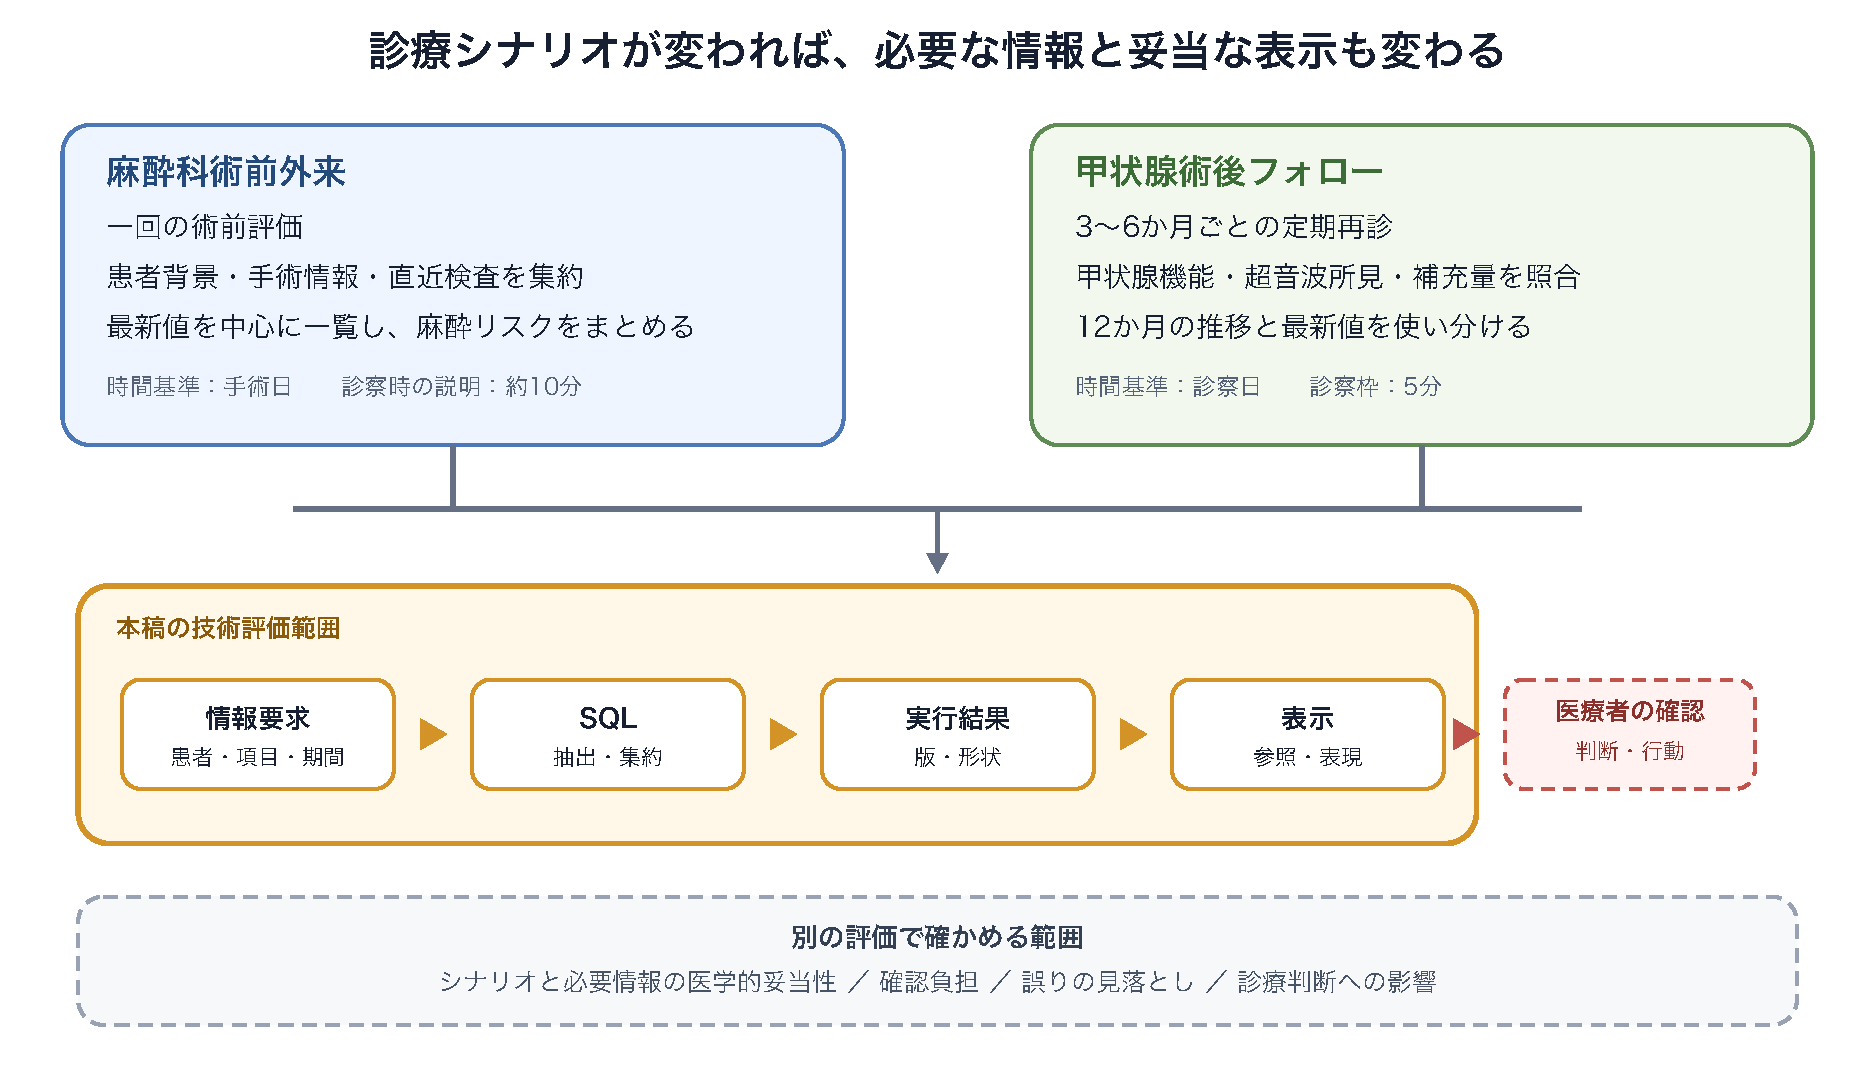
\includegraphics[width=\linewidth]{scenario-to-value.pdf}
  \caption{診療シナリオから利用者価値までの関係と、本稿の技術評価範囲。二つのシナリオは設計例であり、正式評価ケースではない。}
  \Description{麻酔科術前外来と甲状腺術後フォローでは、時間基準、必要情報、表示方法が異なる。両者から情報要求、SQL、実行結果、表示へ進む過程を本稿の技術評価範囲として囲み、医療者の確認と判断、医学的妥当性、確認負担、診療判断への影響を別の評価範囲として示している。}
  \label{fig:scenario-to-value}
\end{figure}

\subsection{利用者価値までの因果関係}

生成臨床UIが医療者へ価値を返すまでには、少なくとも三つの条件がある。まず、専門家が診療シナリオに必要な質問、情報、完了条件を定める。次に、システムがその情報要求を正しいデータ取得と表示へ変換する。最後に、医療者が表示を使って必要な情報を確認し、診療タスクを行う。本稿が直接測るのは二番目である。

層間整合性が高ければ確認負担や見落としが減るとは、本結果だけでは言えない。層間整合性は、妥当な情報を使ったUXを評価する前提になる。対象患者や期間を誤った画面を使って、操作時間や好みだけを測っても、診療タスクに適したUIかは判断できないためである。今後は、専門家が確認したシナリオと合成症例を使い、誤った更新の受理、妥当な更新の受理、問題箇所の特定、修復、確認時間、操作数、認知負荷を分けて測る必要がある。

\subsection{何を情報の誤りと呼ぶか}

情報の正しさには複数の段階がある。本稿では、元データの記録内容が事実か、診療シナリオのタスク定義が医学的に適切か、表示を見た医療者の判断が正しいかを評価しない。本稿が扱う\term{情報の誤り}は、定められた情報要求に対して、画面へ届いた情報が患者、項目、期間、集約、情報源、表示方式、接続、版のいずれかで一致しない状態である。層間不整合は、この誤りを成果物間の関係として特定したものである。

この定義により、SQLが実行できない失敗と、SQLは実行できるが別の情報を返す失敗を区別できる。前者は局所検査で見つけられる。後者を見つけるには、情報要求とSQL、SQLと実行結果、実行結果と表示の対応を検査しなければならない。

\section{層間整合性の定義}

\subsection{対象とする情報の流れと検知の仕組み}

本研究は、情報要求、SQL、実行結果、表示部品の4層を扱う。情報要求は、対象患者、対象項目、期間、集約、情報源、期待する表示方式を含む。SQLは要求をデータベース操作へ変換する。実行結果はSQL、入力、実行時点に対応する版を持つ。表示部品は、結果を参照し、その形状に適した方法で提示する。

\begin{figure}[t]
  \centering
  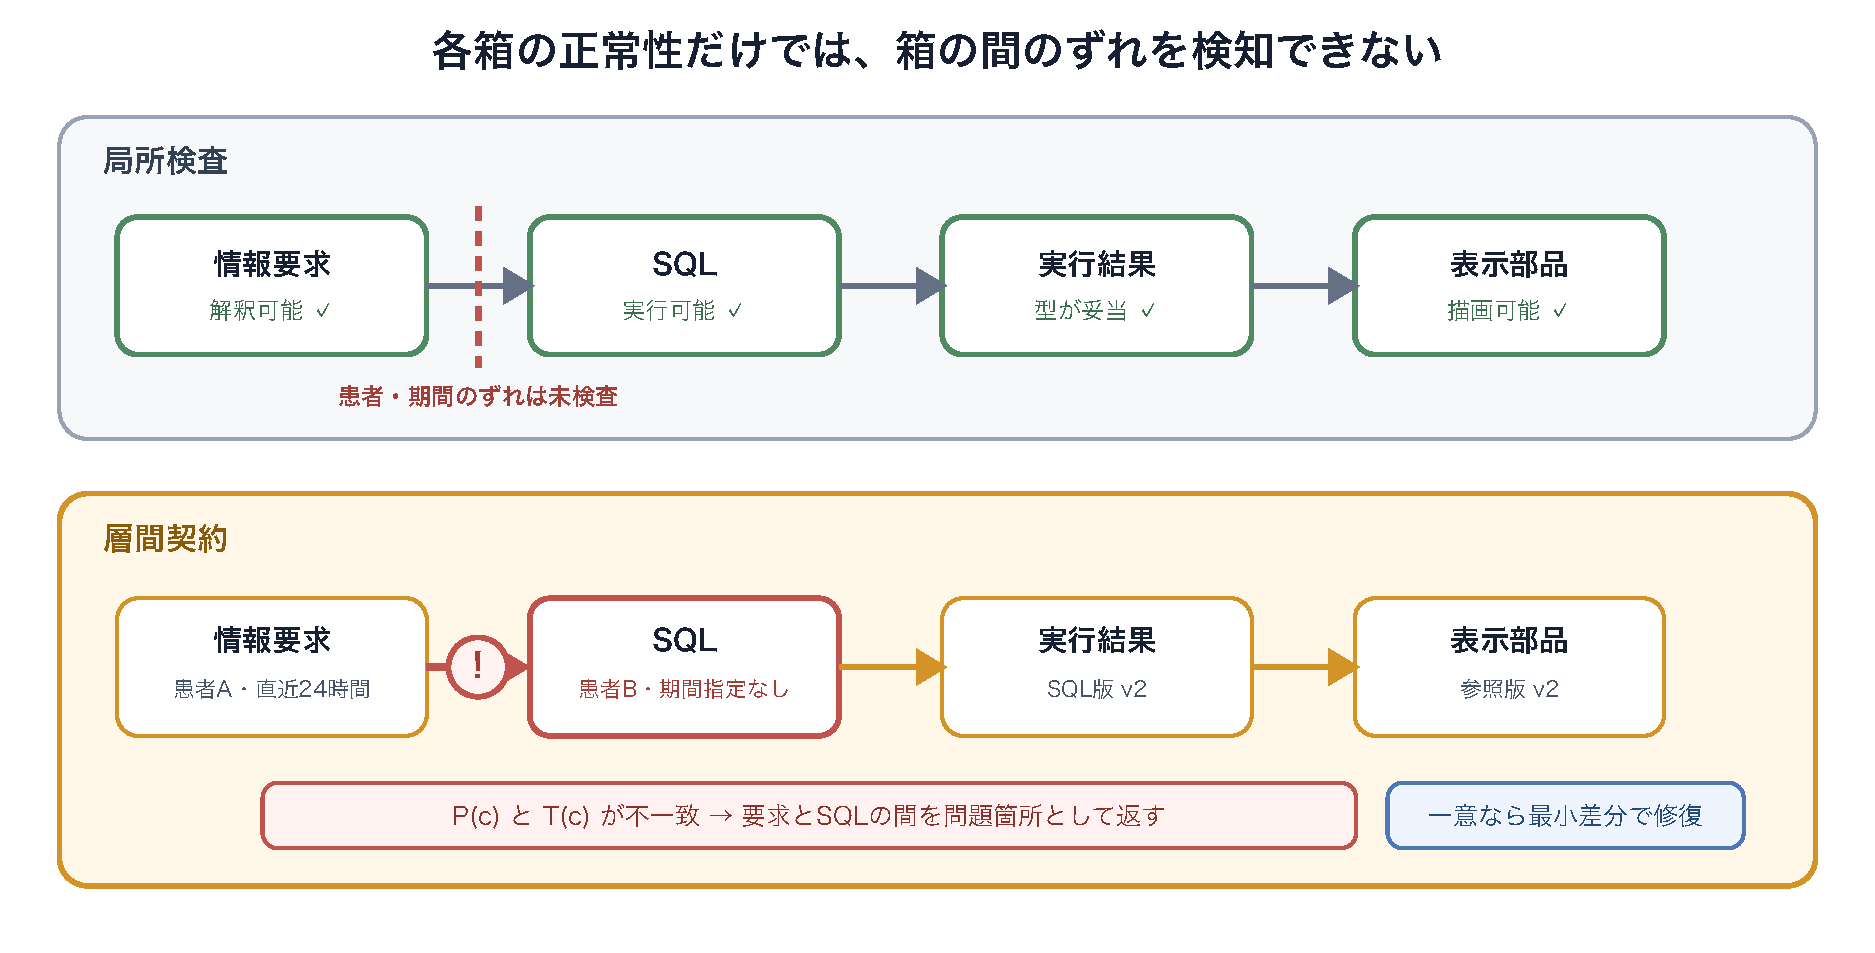
\includegraphics[width=\linewidth]{detection-mechanism.pdf}
  \caption{局所検査と層間契約の違い。層間契約は意味キーと版を隣接層で比較するため、各成果物が単独で有効でも要求と異なる情報を検知できる。}
  \Description{上段では、情報要求、SQL、実行結果、表示部品がそれぞれ局所検査を通過するが、情報要求とSQLの患者と期間のずれが未検査になる。下段では、情報要求が患者Aと直近24時間を指定するのに対し、SQLは患者Bを参照し、期間も指定していない。このため、患者と期間の述語が不一致となり、問題箇所が情報要求とSQLの間に特定される。}
  \label{fig:detection-mechanism}
\end{figure}

図\ref{fig:detection-mechanism}に、層間不整合を検知できる仕組みを示す。局所検査は各箱の内部だけを見る。層間契約は、情報要求から抽出した意味キーをSQL解析結果と比べ、SQLの版を実行結果と比べ、結果の参照先と形状を表示部品と比べる。不一致があれば、失敗した述語と、その述語が結ぶ二つの成果物を返す。同じ意味を表す値を成果物境界で比較できることが検出を支える。グラフ探索の性質によるものではない。

更新候補$c$が層間整合性を満たすとは、要求とSQLの意味が一致し、SQLと実行結果の版が一致し、結果と表示部品の参照および表示方式が一致することとする。これを次の述語の論理積で表す。

\begin{equation}
I(c)=P(c)\land D(c)\land T(c)\land A(c)\land S(c)\land V(c)\land L(c)\land R(c)
\end{equation}

$P$は患者、$D$は項目、$T$は期間、$A$は集約、$S$は情報源、$V$は表示方式、$L$はデータと表示の接続、$R$はSQLと実行結果の版の一致を表す。候補生成では、妥当候補は8述語をすべて満たし、不整合候補は一つだけ満たさないようにする。

\subsection{8種類の不整合}

表\ref{tab:mutations}に不整合の定義を示す。対象患者の不整合では、要求側の患者を保ったままSQLの患者条件を別の候補へ変える。対象項目では、要求と異なる列または集約対象を取得する。期間では、要求の時点や期間に対応する条件を変える。集約方法では、件数、最大、最小、平均などを別の演算へ置き換える。

\begin{table}[t]
  \caption{評価で生成する8種類の層間不整合}
  \label{tab:mutations}
  \begin{tabularx}{\linewidth}{lYY}
    \toprule
    種類 & 変更するもの & 単独では通り得る検査 \\
    \midrule
    対象患者 & SQLの患者条件 & 構文、読み取り専用、実行 \\
    対象項目 & 取得列または集約対象 & 構文、実行、結果型 \\
    期間 & 時点・期間条件 & 構文、実行 \\
    集約方法 & 件数、最大、最小、平均など & 構文、実行、結果型 \\
    情報源 & 参照表 & 構文、実行 \\
    表示方式 & 結果を示す部品の種類 & UI構造、描画 \\
    接続 & 部品が参照するデータ取得 & 個別ノードの型 \\
    古い結果 & SQL更新後の結果版 & SQL実行可能性、結果型、描画 \\
    \bottomrule
  \end{tabularx}
\end{table}

情報源の不整合では、要求が対応付けられた表とSQLの参照表をずらす。表示方式では、SQL、実行結果、列、値を保ったまま、基準が数値カードならデータフレーム表示へ、基準がデータフレーム表示なら別の表部品へ変える。接続では、表示部品が別のデータノードを参照する。古い結果では、SQLを更新しても実行結果の版を以前のまま残す。

これらは臨床現場で観測したエラー頻度の分類ではない。どの関係を検査する必要があるかを測定可能にするための故障モデルである。各候補には一種類だけを注入するため、結果は複合故障への性能を示さない。

\section{評価基盤}

\subsection{基準ケースの構築}

入力はEHRSQL-2024の回答可能な質問と正解SQLである。回答不能ケースは正解SQLから基準UIを構築できないため、主評価から除外し、件数を記録する。正解SQLはMIMIC-IV Demo v2.2のSQLiteデータベースへ読み取り専用で実行する。書き込みを含む文、複数文、許可しない構文は実行前に拒否し、SQLごとの実行上限を5秒とした。

実行結果が単一値なら数値カード、複数行または複数列ならデータフレーム表示を基準とする。空結果は除外せず、列構造を持つ結果として扱う。基準ケースは、質問テンプレートから抽出した意味スロット、SQLの解析結果、結果形状、データノード、表示部品、各成果物の版を保持する。

同じ質問テンプレートとSQL構造を共有するケースを更新前後として組み合わせる。この組から、すべての関係を同時に更新した妥当候補と、一つの関係だけを壊した不整合候補を作る。同じ質問形式から派生する候補は独立ではないため、後の統計処理では質問テンプレートを再標本化の単位とする。

\subsection{独立したオラクル}

候補生成と正解判定は別の処理で実装した。オラクルは、質問テンプレートの意味スロット、SQLの解析結果、実行結果の形状と版、データノードと表示部品の参照を照合する。候補生成器が付けた期待ラベルとオラクルの判定が一致しない場合、評価を停止する。

完成したJSONの完全一致を正解としない。安定ID、順序、表示文言など、意味を変えない差を許すためである。一方、画面の見た目が同じでも、別患者、異なる期間、古い結果を参照する候補は不整合とする。この設計により、表層的な一致と意味上の対応を分ける。

\subsection{4種類の検査条件}

同一候補を表\ref{tab:conditions}の4条件へ入力する。\condition{局所検査}は、SQLが読み取り専用で実行可能か、成果物がスキーマに適合するか、表示部品が描画可能な型かを個別に確認する。\condition{成果物契約}は、SQL、実行結果、表示部品のそれぞれに条件を追加するが、情報要求から表示までを横断して照合する関係群は持たない。

\condition{グラフ契約}では、質問テンプレート、SQL、結果、データノード、表示部品をノードとする。患者、項目、期間、集約、情報源、版、参照、表示方式の関係は、辺として保持する。候補更新後に、影響を受ける関係を再評価する。\condition{平坦契約}は、グラフと同じ意味スロットと対応関係を一枚のサイドカー表に保持し、同じ述語を検査する。二条件の内容をそろえることで、確認内容の効果とグラフ形式の効果を分ける。

\begin{table}[t]
  \caption{比較する4種類の検査条件}
  \label{tab:conditions}
  \begin{tabularx}{\linewidth}{lYYY}
    \toprule
    条件 & 個別成果物 & 層間関係 & 保存形式 \\
    \midrule
    局所検査 & 基本検査 & なし & 各成果物 \\
    成果物契約 & 詳細検査 & 一部 & 各成果物 \\
    グラフ契約 & 詳細検査 & すべて & ノードと辺 \\
    平坦契約 & 詳細検査 & すべて & 一枚の表 \\
    \bottomrule
  \end{tabularx}
\end{table}

\subsection{診断と一回の修復}

検査が候補を拒否した場合、失敗した述語と関係する成果物を診断として返す。特定率は、注入した不整合の種類を診断が正しく示した割合とする。検出しただけで、場所または種類を誤った場合は特定成功に数えない。

修復には診断を一回だけ使い、基準契約から一意に定まる値を戻す。たとえば、表示部品の参照先、結果版、表示方式は、対応する契約から復元する。修復後の候補をオラクルと同じ整合性述語で再検査し、すべてを満たした場合だけ成功とする。探索、複数回の試行、生成モデルによる書き換えは行わない。

\subsection{評価手順}

図\ref{fig:protocol}に評価手順を示す。開発用データでは、異なる質問テンプレートを優先した50件でSQL実行と基準ケースへの変換を確認した。調整確認用データでは、不整合ごとの候補数、質問テンプレート数、ラベル一致、機微情報を保存しない条件を確認した。列順の不整合が生成できなかったため、テスト分割を見る前に表示方式の不整合へ置き換えた。他の不整合、指標、分析、停止条件は維持した。

\begin{figure}[t]
  \centering
  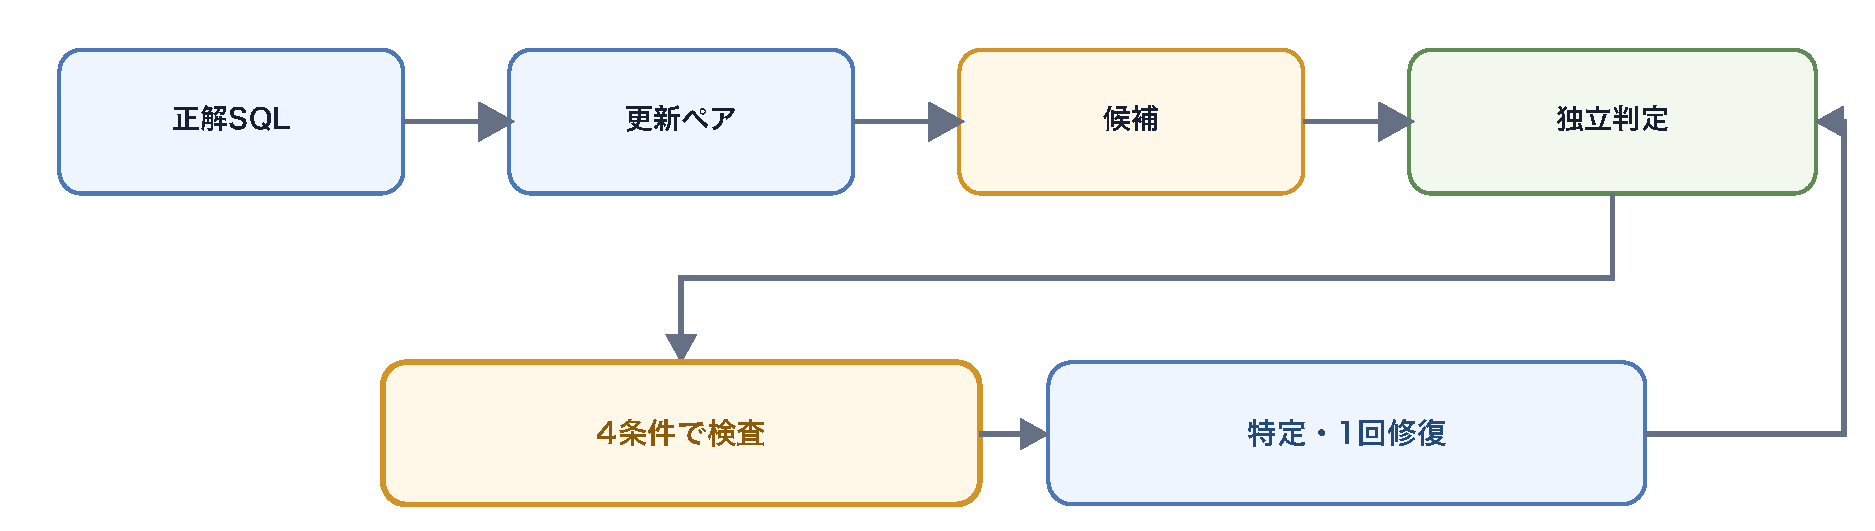
\includegraphics[width=\linewidth]{evaluation-protocol.pdf}
  \caption{基準ケースの構築から候補生成、検査、診断、修復までの評価手順。}
  \Description{正解SQLから基準ケースを作り、更新ペア、妥当候補、不整合候補を順に作る。独立オラクルで候補を確認し、四条件で検査して一回だけ修復する流れを示す。}
  \label{fig:protocol}
\end{figure}

調整確認用データで事前基準を満たした後、評価コード、設定、分析をGit commit \texttt{baa82075b6bf}で固定した。固定後、テスト分割を一度だけ実行した。評価中に生成モデルや外部モデルは呼び出していない。

\subsection{指標と統計分析}

主指標は\term{不整合流出率}と\term{妥当更新受理率}である。不整合流出率は、注入した不整合候補のうち検査が受理した割合であり、低いほどよい。妥当更新受理率は、すべての関係を正しく更新した候補のうち受理した割合であり、高いほどよい。副次指標として、問題箇所の特定率、一回の修復成功率、候補当たりの平均検証時間を測る。

条件差は同じ候補に対する対応差として計算する。95\%信頼区間は、質問テンプレート単位のクラスターブートストラップを10,000回行って求める。再標本化の単位を質問テンプレートとするのは、同じSQL構造と変異規則を共有する派生候補を独立例として扱わないためである。

\subsection{データ管理と再現性}

公開成果物には、生データ、質問文、正解SQL、患者ID、患者単位の結果値を保存しない。保存するのは、ハッシュ化したケース識別子、入力と候補のチェックサム、不整合の種類、判定、診断、修復、集計、実行環境である。正式結果はJSONとJSON Linesで固定し、別の処理でTSVへ変換して件数、主要指標、95\%信頼区間を再計算した。再集計値は元の集計と一致した。

\section{結果}

\subsection{基準ケースと候補}

テスト分割には1,167件があり、正解SQLを持つ回答可能ケース934件を対象とした。回答不能233件は主評価から除外した。934件すべてで正解SQLの実行と基準成果物の構築に成功し、82件は列構造を持つ空結果だった。134種類の質問テンプレートから763組の更新前後ペアを作った。各ペアについて妥当候補と不整合候補を作り、4条件へ入力したため、検査回数は$763\times2\times4=6,104$回となった。候補ラベルと独立オラクルの不一致は0件だった。

不整合の生成数は、対象患者52件、対象項目55件、期間106件、集約方法34件、情報源134件、表示方式134件、接続129件、古い結果119件であり、合計763件だった。患者、項目、期間、集約では、意味を一つだけ変えられる代替SQLがない場合に候補化を見送った。この生成可否はデータと質問形式に依存するため、8種類の件数は均等ではない。

\subsection{RQ1：局所検査を通過する不整合}

局所検査は8種類すべての不整合候補を受理し、不整合流出率は100.00\%だった。各候補では、SQLを読み取り専用で実行でき、結果と表示部品も個別には有効になるよう構成している。この結果は、対象患者や期間の誤りに加え、表示方式、接続、古い結果も、構文、スキーマ、描画可能性を個別に確かめるだけでは検出できないことを示す。

成果物契約の流出率は不整合の種類で異なった。表\ref{tab:mutation-results}に示すように、情報源、表示方式、古い結果はすべて拒否した。一方、患者、項目、期間、集約の不整合は92.73\%から98.08\%が流出し、接続の不整合はすべて流出した。各成果物の内部に記述できる条件は検査できても、要求とSQL、データノードと表示部品のように成果物をまたぐ対応が弱点として残った。

\begin{table}[t]
  \caption{不整合の種類別に見た成果物契約の流出率}
  \label{tab:mutation-results}
  \begin{tabularx}{\linewidth}{Yrrr}
    \toprule
    種類 & 生成数 & 流出数 & 流出率 \\
    \midrule
    対象患者 & 52 & 51 & 98.08\% \\
    対象項目 & 55 & 51 & 92.73\% \\
    期間 & 106 & 103 & 97.17\% \\
    集約方法 & 34 & 33 & 97.06\% \\
    情報源 & 134 & 0 & 0.00\% \\
    表示方式 & 134 & 0 & 0.00\% \\
    接続 & 129 & 129 & 100.00\% \\
    古い結果 & 119 & 0 & 0.00\% \\
    \midrule
    合計 & 763 & 367 & 48.10\% \\
    \bottomrule
  \end{tabularx}
\end{table}

\subsection{RQ2：4条件の検出、受理、特定}

主結果を表\ref{tab:main-results}に示す。グラフ契約と平坦契約は、不整合候補763件をすべて拒否し、妥当候補763件をすべて受理した。局所検査との差は$-100.00$ポイントで、95\%信頼区間は$[-100.00,-100.00]$だった。成果物契約との差は$-48.10$ポイントで、95\%信頼区間は$[-49.56,-46.53]$だった。妥当更新受理率は4条件すべて100.00\%で、条件差は0だった。

\begin{table}[t]
  \caption{4条件の主結果と副次結果}
  \label{tab:main-results}
  \begin{tabularx}{\linewidth}{Yrrrr}
    \toprule
    条件 & 不整合流出 & 妥当受理 & 特定 & 平均時間 \\
    \midrule
    局所検査 & 763/763 & 763/763 & 0/763 & 2.152 ms \\
    成果物契約 & 367/763 & 763/763 & 387/763 & 7.441 ms \\
    グラフ契約 & 0/763 & 763/763 & 763/763 & 9.339 ms \\
    平坦契約 & 0/763 & 763/763 & 763/763 & 9.296 ms \\
    \bottomrule
  \end{tabularx}
\end{table}

成果物契約は、不整合396件を拒否したうち387件で注入箇所を正しく特定し、特定率は50.72\%だった。グラフ契約と平坦契約は763件すべてで種類と箇所を特定した。両条件の判定不一致は0件であり、不整合流出率の差も0ポイントだった。候補当たりの平均検証時間は、局所検査2.152 ms、成果物契約7.441 ms、グラフ契約9.339 ms、平坦契約9.296 msだった。この評価環境では、層間関係を検査する二条件の時間差は0.043 msだった。

\subsection{RQ3：一回の修復}

局所検査は不整合を検出しないため、修復を試行しなかった。成果物契約は拒否した396件へ一回の修復を試み、387件が独立オラクルのすべての述語を満たした。試行した候補に対する成功率は97.73\%である。残る9件は一回の修復後も整合性を満たさなかった。

グラフ契約と平坦契約は、全763件の不整合を特定した。一回の修復後には、全件が整合性を満たした。両条件で不要な拒否はなく、妥当候補に修復は適用されなかった。この100\%は、単一故障、既知の契約、決定的な修復規則という本評価の範囲で得た結果であり、自然発生する複合的な生成誤りへの一般化を示さない。

\section{考察}

\subsection{SQLの正しさから、要求した情報を表示へ届ける過程の正しさへ}

局所検査では、8種類すべての不整合が通過した。SQL、結果、表示部品がそれぞれ正常に動くことは必要だが、それだけでは医療者へ正しい情報を返せない。生成臨床UIの評価単位はSQLや画面の単体ではなく、診療シナリオから情報要求を定め、データを抽出し、結果を表示する一連の過程である。

この枠組みでは、SQL生成性能の改善は過程の一部に位置付く。正しいSQLが一度得られても、増分更新で患者、期間、結果版、表示先がずれれば、最終画面は要求へ答えない。逆に、見た目が整った画面も、取得元を確認できなければ妥当なUXとは判定できない。生成UI研究では、表層の品質、成果物の実行可能性、情報の来歴、利用者が行う確認を分け、最後に同じ診療タスクへ結び直す必要がある。

\subsection{なぜ層間契約は誤りを検知できたか}

成果物契約は情報源、表示方式、古い結果をすべて拒否したが、患者、項目、期間、集約の大半と接続のすべてを見逃した。前者は許可表、結果形状、版などを一つの成果物内に記述できる。後者は、要求とSQL、またはデータノードと表示部品を比較しなければ分からない。

層間契約は、患者、項目、期間、集約、情報源、表示方式を意味キーとして保持し、版と参照先も含めて隣接する成果物間で比較した。SQLの再実行にとどまらず、要求から受け継ぐべき値が境界を越えて同じかを判定できた。不一致を関係の位置へ結び付けるため、拒否だけでなく問題箇所の特定と修復にも使えた。この検知メカニズムを示すことが、流出率0\%という結果の解釈に必要である。

\subsection{シナリオ差が示す医療固有の要件}

麻酔科術前外来と甲状腺術後フォローの差は、臨床UIに単一の正解表示を置きにくい理由を示す。術前外来では、広い患者背景と直近検査を一回の評価へ集約する。甲状腺術後フォローでは、限られた検査と処方の時間変化を繰り返し比較する。同じ項目でも、最新値が必要な場面と推移が必要な場面があり、基準日も手術日と診察日で異なる。妥当なUIは、診療シナリオとタスクから決まる。

医療では、情報が表示されたかだけでなく、誰の、何の、いつの情報かが判断材料になる。別患者、誤った期間、古い結果の表示は、画面の小さな不具合として扱えない。専門家が定めた必要情報、安全関連情報、完了条件と結び付け、来歴と更新時点を確認できる設計が要る。ただし、本評価は二つのシナリオの医学的妥当性や、層間契約が臨床上の誤りを減らすかを実証していない。シナリオは設計要件を具体化し、次の評価で何を専門家へ確認すべきかを示す役割を持つ。

\subsection{関係の内容が結果を分けた}

グラフ契約と平坦契約は、判定、問題箇所の特定、一回の修復で同じ結果を得た。検出性能について言えるのは、8種類の関係を明示的に保持して検査すれば、保存形式がグラフでも表でも同じ候補を拒否できたということまでである。グラフ形式そのものを安全性や性能の根拠にはできない。

この否定的結果は、中間表現を評価するときに、保存形式と利用者へ提供する機能を分ける必要があることを示す。グラフは影響範囲の探索、部分更新の伝播、関係の可視化に使える可能性がある。本評価は、その編集しやすさや説明の分かりやすさを測っていない。今後の比較では、同じ最小単位の情報と修復操作を両条件に与え、層間の経路をグラフとして提示することが、医療者による問題箇所の特定と修復を支えるかを測るべきである。

Jelly、Bridging Gulfs、SimStepは、中間表現を利用者が意図を確かめ、生成物を編集する接点として用いている\cite{cao2025jelly,park2026bridging,kaputa2026simstep}。本研究は、この接点に保持する関係を実行結果と表示まで検査できることを、データ駆動型システムの設計要件として提案する。中間表現の価値は、その構造だけでは決まらず、利用者の確認とシステムの実行をどの関係で結ぶかにある。

\subsection{検知を利用者価値へつなぐ}

層間契約による検出成功は、利用者便益そのものではない。本稿の結果から直接言えるのは、既知の単一不整合を表示前に止め、問題箇所を機械可読な形で返せたことまでである。この能力を医療者へ還元するには、診断を更新対話の一部として提示し、利用者が受理、拒否、部分修正を選べるようにする必要がある。

たとえば「無効なUI」とだけ示すより、「要求の患者とSQLの患者条件が一致しない」「表示部品が更新前の結果版を参照している」と示せば、確認範囲を限定できる可能性がある。ただし、診断が確認時間を短くするか、誤った更新の受理を減らすか、妥当な更新まで過剰に拒否させないかは、人を対象とする比較で確かめなければならない。最終画面だけを示す条件と、同じ画面に層間の経路と診断を加える条件を比べ、不正更新の誤受理、妥当更新の受理、問題箇所の特定、意味的に正しい修復、作業時間、認知負荷を分けて報告する。

生成システムの提案を利用者が受理、拒否、交渉する過程を扱った研究\cite{sivaraman2023ignore}を踏まえると、診断表示の評価では正答率だけをまとめてはいけない。不正更新と妥当更新を一つの正答率に混ぜず、不正更新の誤受理と妥当更新の受理を分けて測る。層間情報が識別を助けたのか、単に拒否を増やしたのかを区別するためである。

\subsection{修復と人の判断を分ける}

層間関係をすべて持つ二条件は、既知の単一故障763件を一回で修復した。契約から正しい値が一意に定まる患者条件、参照先、結果版、表示方式では、最小差分を機械的に戻せる。この結果から、検査を拒否判定だけで終わらせず、修復候補へ変換できることが分かる。

自然言語要求が曖昧な場合、臨床的な表示粒度を選ぶ場合、複数の成果物が同時に変わった場合は、一意に修復できない。生成UIは、機械的に修復できる関係、複数候補を人へ示す関係、専門家が決める関係を区別する必要がある。100\%の修復成功率は自動修復の一般的な安全性を示さず、既知の契約から一意に戻せる範囲を示している。

\subsection{高い正確性を求める他領域への移行}

情報要求からデータを取得して画面を生成する仕組みは、医療以外にも金融、航空、産業設備などで使われ得る。これらの領域でも、実行可能な問い合わせと描画可能な画面だけでは、対象、期間、情報源、版の一致を保証できない。層間契約という考え方は移せる可能性がある。

移せるのは検査の構造であり、医療向けの8種類をそのまま使えるとは限らない。領域ごとに、誰が何を判断するのか、誤った情報がどの作業へ影響するのか、どの関係を機械的に検査し、どこから人の判断へ渡すのかを定義する必要がある。CHIに対する本稿の主張は、生成物の品質評価に、利用者のタスクから最終表示までの追跡と診断を加えることである。

\section{制約と倫理}

第一に、本評価の不整合は決定的な規則で一つずつ注入したものであり、生成モデルが自然に起こすエラーの分布を表さない。単一故障で100\%を得た条件が、複合故障、曖昧な要求、未知の表示部品でも同じ性能を持つとは限らない。今後は、固定した検査を自然発生候補へ適用し、不整合分類にない失敗を質的に調べる必要がある。

第二に、正解SQLを出発点としているため、Text-to-SQLモデルの初回生成誤りを含まない。実運用では、質問の解釈とSQL生成も誤り得る。本結果は、正しい基準が得られた後の増分更新に範囲を限定する。質問からSQLを生成する段階を含める場合は、棄権、複数解釈、SQLの臨床的妥当性を別に評価する必要がある。

第三に、MIMIC-IV Demo v2.2とEHRSQL-2024の質問テンプレートだけを使った。麻酔科術前外来と甲状腺術後フォローは問題設定を説明する設計例であり、正式評価ケースではない。結果形状や利用可能な代替条件により、不整合ごとの候補数は異なる。他の診療シナリオ、データモデル、複数施設、複雑な可視化、複数データ源をまたぐ更新へ結果を一般化できない。

第四に、グラフ契約と平坦契約は同じ対応内容を持つよう意図的に実装した。この比較は保存形式だけを分けるためのものであり、大規模な関係の編集しやすさ、実装保守性、説明の分かりやすさを比較していない。検証時間も一つの実装と環境で測った値であり、形式一般の性能差として解釈できない。

第五に、本研究は匿名化済み公開デモデータ上の技術評価である。正解SQLは技術的な基準であり、表示内容の医学的妥当性を専門家が確認した正解ではない。層間整合性が確認負担、誤った更新の受理、診療判断へ与える影響も測っていない。臨床上の安全性、診療判断の正確さ、使いやすさ、認知負荷、臨床転帰、実運用、他施設への一般化は評価していない。人を対象とする評価は、倫理審査と実施許可、募集、同意、撤回、データ管理を確認した後の別研究とする。

公開成果物には、質問文、正解SQL、患者ID、患者単位の結果値を含めない。MIMIC-IV DemoとEHRSQL-2024の利用条件と出典を明記し、公開可能なチェックサム、分類、判定、集計だけを再現資料へ含める。

\section{結論}

診療シナリオに適したUIを生成するには、必要な情報をSQLで取得できるだけでなく、その要求が実行結果と表示まで保たれなければならない。本研究は、この過程で起こる層間不整合を8種類として定義し、公開デモデータ上で決定的に生成して、4種類の検査条件を同一候補上で比較した。

763組の更新前後ペアを使った6,104回の検証では、局所検査が不整合をすべて受理し、成果物契約も48.10\%を受理した。グラフ契約と同じ内容を持つ平坦契約は、不整合をすべて拒否し、妥当な更新をすべて受理した。両者の結果に差がなかったため、本評価範囲では、検出を支えたのはグラフ形式そのものではなく、患者、項目、期間、集約、情報源、表示方式、接続、版の関係を実行可能な契約として保持したことだと解釈できる。

継続的な更新を前提に生成UIを設計するには、最終画面の見た目と個別成果物の妥当性に加えて、診療シナリオ由来の情報要求から表示までの来歴を検査し、問題箇所を説明できる必要がある。本研究は、妥当な臨床UXを評価する前に満たすべき技術条件と、その検知メカニズムを示した。次の課題は、専門家が確認したシナリオへ適用し、層間診断が誤った更新の受理、問題特定、修復、確認負担へ与える影響を、人を対象とする評価で確かめることである。

\bibliographystyle{ACM-Reference-Format}
\bibliography{references}

\end{document}
